\section{System Design}
\label{sec:system}

This section presents the system design and implemetation of
\name.

\subsection{Centralized control of \name}
\label{subsec:system:centralized}

\begin{figure}[t]
  \centering
  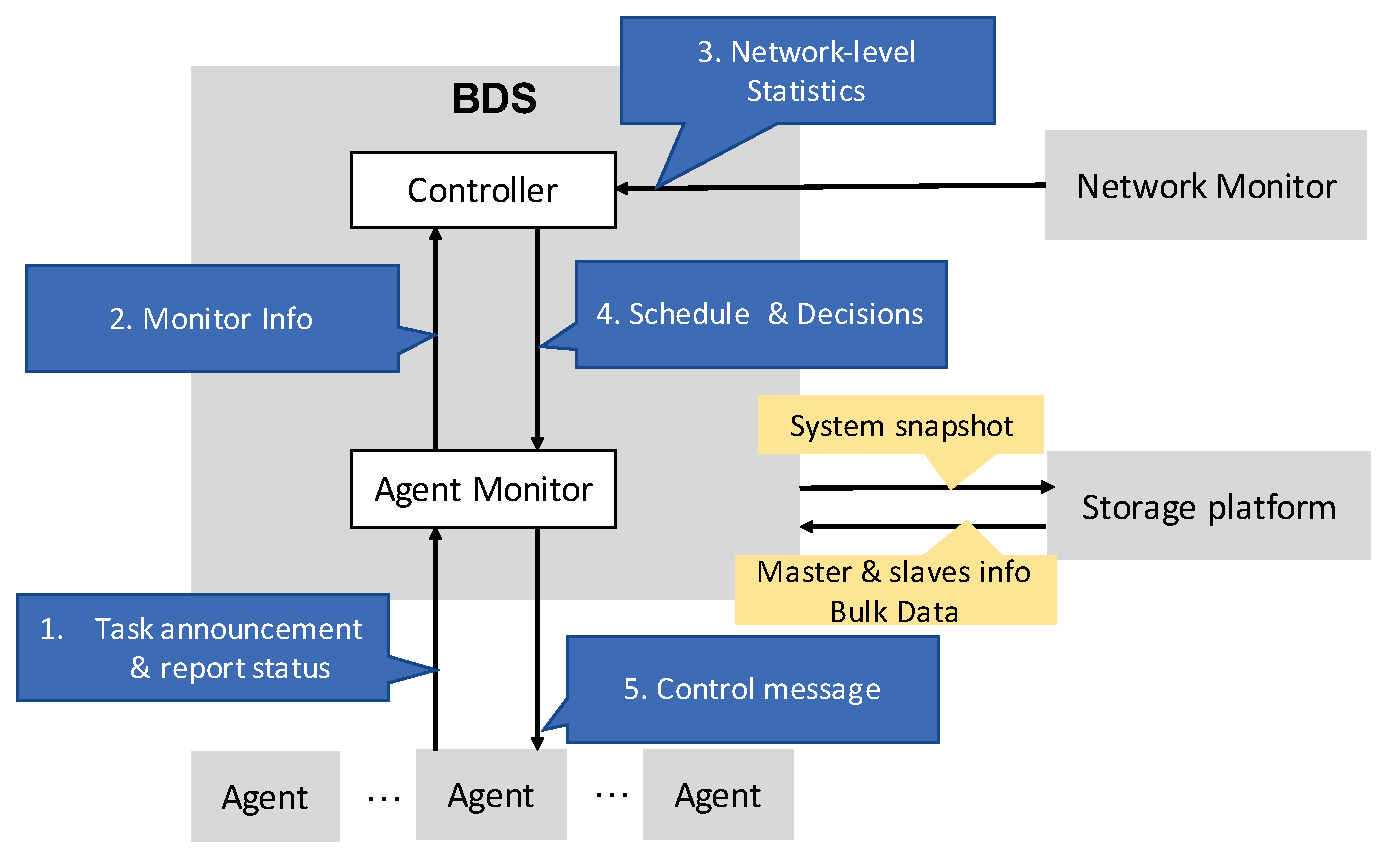
\includegraphics[width=3in]{images/implementation_v4.eps}
  \tightcaption{Interfaces of \name's centralized control.}
% \jc{please add the step of network monitor. see the new text}\jc{where are servers? avoid notions never defined before like "task announcement"}
  \label{fig:implementation}
\vspace{-0.4cm}
\end{figure}
%\vspace{-15pt}

\name periodically (by default, every three seconds) updates the
routing and scheduling decisions in a centralized fashion.
Figure \ref{fig:implementation} outlines the workflow in each
three-second cycle.
\begin{enumerate}
\item It starts with the {\em Agent}, running local on each server,
checking the local states, including data block delivery status
(which blocks have arrived, and which blocks are outstanding),
server availability, and disk failures, etc.
\item These statistics are then wrapped in a {\em control message},
and sent to the centralized {\em \name Controller} via an efficient
messaging layer called {\em Agent Monitor}.
\item The \name Controller also receives network-level statistics
(the bandwidth consumption by latency-sensitive traffic and the
utilization on each inter-DC link) from a {\em Network Monitor}.
\item On receiving the updates from all Agents and the Network
Monitor, the \name Controller runs the centralized decision-making
algorithm (\Section\ref{sec:logic}) to work out the new scheduling
and routing decisions, and sends the difference between the new
decision and the previous one to the per-server local Agent via
the Agent Monitor messaging layer.
\item Finally, the Agent allocates bandwidth for each data transfer,
and carries out the actual data transfers according the Controller's
routing and scheduling decisions.
\end{enumerate}


\name uses two additional optimizations to make the workflow
more efficient.
\begin{itemize}
\item \emph{Blocks merging}.
To reduce the computational scale and achieve more efficient
transmissions, \name merges the blocks with the same source and
destination into one subtask. Its benefits are two-fold: (1) it
significantly reduces the number of pending blocks in each
scheduling cycle, thus reducing the computational cost of the
centralized decision-making logic; and (2) it reduces the number
of parallel TCP connections between servers, which could
otherwise reduce link utilization and degraded performance.
\item \emph{Non-blocking update}.
To avoid being blocked by the controller's decision-making logic,
each local Agent  keeps the ongoing data transmissions alive while
the Controller runs the centralized decision-making logic.
Similarly, the Controller takes this into account by speculating
the changes in data delivery status while the decisions are being
re-calculated, and using these speculated data delievery status as
the input of the centralized logic.
\end{itemize}

\NEW{
\subsection{Dynamic bandwidth separation}
}
\label{subsec:system:separation}

To guarantee clean separation of bandwidth between inter-DC
bulk-data multicasts and delay-sensitive traffic, \name Network
Monitor monitors the aggregated bandwidth usage of all
latency-sensitive flows on each inter-/intra-DC link, and
dynamically allocates the bandwidth of each inter-DC multicast
transfer. To protect delay-sensitive flows from being negatively
affected by bursty bulk-data transfers, \name uses 80\% link
utilization as a ``safety threshold'', i.e., the total bandwidth
consumption of bulk-data transfers cannot exceed 80\% of the link
capacity on any link, and dynamically decides the sending rate
of each data transfer.

The key advantage of \name's dynamic bandwidth separation is that it
efficiently allocates bandwidth in a centralized manner,
similar~\cite{kumar2015bwe} in the transport layer. The traditional
techniques (e.g.,~\cite{kumar2015bwe}) that gives higher priority to
online latency-sensitive traffic can still have bandwidth wastage or
performance interference in the presence of dynamic network
environments~\cite{wang2017toward}. \name, in contrast, dynamically monitors the aggregated
bandwidth of delay-sensitive applications, and calculates the
residual bandwidth to be used by inter-DC multicast while meeting the
safety link utilization threshold. Finally, note that \name optimizes
the application-level overlay, and is thus complementary to
network-layer techniques that improve the WAN performance and
fairness~\cite{chen2012design, kavulya2010analysis, mishra2010towards, reiss2012heterogeneity}.


\subsection{Fault tolerance}
\label{subsec:system:fault}
Next we describe how \name handles the following failures.

\begin{packedenumerate}
\item \emph{Controller failure:} The \name controller is
replicated~\cite{lamport1998part}: if the master controller fails,
another replica will be elected as the new controller. If all
controller replicas are not available (e.g., a network partition
between DCs and the controllers), the agents running in servers will
fallback to the current decentralized overlay protocol as default to
ensure graceful performance degradation.
\item \emph{Server failure:} If the agent on server is still able to
work, it will report the failure state (e.g., server crash, disk
failure, etc.) to the agent monitor in the next cycle. Otherwise, the
servers that selected this server as data source would report the
unavailability to the agent monitor. In either case, the controller
will remove that server from the potential data sources in the next
cycle.
\item \emph{Network partition between DCs:}
If network partition happens between DCs, the DCs located in the same
partition with the controller will work the same as before, while the
separated DCs will fallback to the decentralized overlay network.
\end{packedenumerate}



